\documentclass[a4paper, oneside]{article}
\usepackage{graphicx}
\usepackage{amsthm}
\usepackage{amsmath} 
\usepackage{amssymb}
\usepackage[a4paper,
            bindingoffset=0.2in,
            left=1.75cm,
            right=1.75cm,
            top=1.75cm,
            bottom=1.75cm,
            footskip=.25in]{geometry}
\usepackage[italian]{babel}
\usepackage{pgfplots}
\usepackage{tabularx}
\usepackage{tikz}
\usepackage{wrapfig}
\usepackage{color}
\usepackage[d]{esvect}
\usepackage{svg}
\usepackage{float}
\usepackage{booktabs}
\usepackage{circuitikz}
%\definecolor{page}{rgb}{0.129,0.157,0.212}
%\pagecolor{page}
%\color{white}
\graphicspath{ {./images/} }
\usetikzlibrary{shapes.geometric}
\usetikzlibrary{datavisualization}
\usetikzlibrary{datavisualization.formats.functions}
\usetikzlibrary{patterns}
\pgfplotsset{width=10cm,compat=1.18}

\title{Esperienza Amplificatore Operazionale}
\author{Gruppo 28 \\ Checchi Alessia, Nuti Giulia, Miliani Tommaso, Ronchi Mattia, Tempestini Ginevra}
\date{26 Marzo 2026}

\begin{document}
\newtheoremstyle{theoremEnv}
                {}          % Space above
                {}          % Space below
                {\slshape}  % Body font
                {}          % Indent amount
                {\bfseries} % Head font
                {.}         % Punctuation after head
                {\newline}  % Space after theorem head
                {}          % Theorem head spec
\theoremstyle{theoremEnv}

\newtheorem{definition}{Definizione}[section]
\newtheorem{theorem}{Teorema}[section]
\newtheorem{lemma}{Proposizione}[section]
\newtheorem{observation}{Osservazione}[section]
\newtheorem{corollary}{Corollario}[theorem]
\newtheorem{example}{Esempio}[section]
\newtheorem{remark}{Enunciato}[section]

\maketitle

\section{Scopo dell'esperienza}
Lo scopo dell'esperienza è lo studio del comportamento di un amplificatore operazionale in configurazione invertente
attraverso due fasi distinte:
\begin{enumerate}
    \item Nella prima fase si intende determinare il guadagno della differenza di potenziale $A_f$ in funzione del
    rapporto tra i resistori scelti $R_f/R_s$. Il valore sperimentale, ottenuto tramite l'analisi della pendenza di
    un fit lineare, sarà confrontato con il valore teorico atteso per verificarne la consistenza.
    Tale analisi permette inoltre di stimare indirettamente la tensione di offset $V_{off}$ tramite il fit lineare.
    \item Nella seconda fase, l'obiettivo è la misurazione della corrente di Bias Ib intrinseca agli
    ingressi dell'amplificatore. Tale misura viene effettuata riconfigurando il circuito come un
    integratore di corrente e analizzando l'evoluzione temporale della tensione d'uscita prodotta
    dalla carica di un condensatore.
\end{enumerate}

\section{Componentistica}
Il circuito è stato assemblato su una breadboard, utilizzando la seguente strumentazione:
\begin{itemize}
    \item Amplificatore operazionale Integrato TL081(niente/B):
componente a singolo canale con ingresso a JFET (FET-input), caratterizzato da una tensione di alimentazione fino a
$\pm$ 15V (con un range massimo totale di 30V), una banda passante in tensione di 3MHz che lega guadagno e frequenza
massima di funzionamento e uno slew rate di 13 V/$\mu$s, che indica la massima velocità con cui l'uscita può variare.
Il datasheet riporta una tensione di offset nominale di circa 3mV e correnti di bias nell'ordine di 30 pA.
(B)Single, 30V, 3MHz, 13-V/$\mu$s slew rate, 3-mV offset voltage, In to V+, FET-input op amp . (niente)Single, 30V,
3MHz, 13-V/$\mu$s slew rate, In to V+, FET-input op amp.
    \item Generatore di tensione Keysight E3659A Dual Output:
utilizzato per fornire l'alimentazione simmetrica $\pm$ 15V necessaria al funzionamento dell'integrato (Pin 7 e Pin 4).
I due canali indipendenti sono stati collegati in serie per definire il potenziale di riferimento comune di massa.
\item Generatore di tensione a singolo canale KAT5VD:
alimentatore stabilizzato con uscita variabile $\frac{1}{15}$ Vdc 5A (corrente massima erogabile in uscita), utilizzato come
sorgente per la tensione di ingresso $V_s$ da amplificare.
\item Resistenze: i valori nominali sono stati verificati sperimentalmente mediante un multimetro digitale prima dell'assemblaggio del circuito. La misura è stata effettuata connettendo i componenti direttamente ai morsetti d'ingresso dello strumento e le incertezze associate ai valori riportati corrispondono alla risoluzione e all'accuratezza garantite dal multimetro.
\begin{itemize}
    \item Resistenza $R_f$ da $(0.996 \pm 0.010) \cdot 10 ^{5} \ \Omega$, con tolleranza 1\%.
    \item Resistenza $R_s$ da $(0.997 \pm 0.010) \cdot 10^{4} \ \Omega$, con tolleranza 1\%.
    \item Resistenza $R_s' = (0.998 \pm 0.010) \cdot 10^{3}\  \Omega$, con tolleranza 1\%.
\end{itemize}
\item Potenziometro multigiro:
da 1 k$\Omega$, utilizzato come partitore di tensione per regolare finemente la tensione $V_s$ fornita
dal generatore KAT5VD, permettendo di ottenere valori piccoli necessari per non saturare l'uscita dell'operazionale.
\item Due Multimetri digitali Goldstar DM-311:
utilizzati per la misurazione diretta delle tensioni. Entrambi gli strumenti sono a $3 \ 1/2$ cifre
(con un conteggio massimo di 1999). L'accuratezza dichiarata dal produttore per la funzione "Volt"
in corrente continua (DC) è di $\pm$ 0.5\% $+$ 1 digit. Per la tensione di ingresso $V_s$, è stata
utilizzata la portata 2V con una risoluzione di 1mV. Per la tensione di uscita $V_0$, è stata
utilizzata la portata 20V con una risoluzione di 10mV.
L'impedenza d'ingresso di 10 M$\Omega$ garantisce che l'inserimento dei multimetri non provochi
effetti di carico significativi sul circuito in esame.
\item Trimmer a tre terminali che si comporta come un potenziometro regolabile di precisione.
\item Multimetro digitale Amprobe LCR55A : utilizzato per misurare la misura diretta della capacità del condensatore, ottenuta collegando direttamente il componente ai terminali dello strumento e leggendo il valore indicato sul display.  Questo multimetro è uno strumento a 3 1/2 cifre (con un conteggio massimo di 1999) con una accuratezza dichiarata dal produttore per la misura di capacità pari a $\pm 1.0\%$ del valore letto + 1 digit. Per la misura è stata utilizzata una portata di 20 nF con una risoluzione di 0.01 nF .
\item Condensatore: utilizzato nella configurazione a integratore per la misura della corrente di bias dell'amplificatore operazionale. Il componente presenta una capacità nominale pari a $\mathcal{C} = 4.70 \pm 0.06$ nF, con un'incertezza pari a 0,06nF, stimata sulla base delle specifiche del multimetro utilizzato per la misura.
\end{itemize}

\section{Parte 1: determinazione dell'amplificazione $A_f$ di un amplificatore operazionale}
\subsection{Apparato sperimentale}
Per la realizzazione di un amplificatore operazionale in configurazione invertente
con guadagno teorico $A_f$, il terminale invertente (pin 2) dell'operazionale
è stato collegato al segnale d'ingresso tramite la resistenza $R_s$. 
La tensione d'ingresso $V_s$ è stata modulata finemente mediante un
potenziometro multigiro da 1 kOhm (caratterizzato da un'escursione
meccanica di 10 giri), interposto tra l'alimentatore a singola
uscita e l'ingresso della resistenza $R_s$. Il sistema di
regolazione dell'ingresso è stato preventivamente tarato
affinché, a fondo corsa orario, la tensione erogata fosse
pari a circa 1.005 V. Questo accorgimento è stato adottato
per garantire che il segnale amplificato in uscita non
superi i $\pm$15V, prevenendo così la saturazione del TL081
e assicurando il corretto funzionamento all'interno del
regime di linearità. Il terminale non invertente (Pin 3)
del circuito integrato è stato posto direttamente a
massa in modo da fissare il riferimento del circuito,
parallelamente il terminale invertente (Pin 2)
è stato collegato all'output dell'amplificatore (Pin 6)
tramite la resistenza di retroazione $R_f$. Per permettere
al TL081 di lavorare in regime lineare evitando
saturazioni premature, il generatore a due canali
è stato configurato per fornire un'alimentazione simmetrica
(collegando in serie le due uscite e riferendo il punto
comune alla massa del circuito) $\pm$15V. La misurazione
della differenza di potenziale in uscita all'amplificatore
operazionale è stata effettuata mediante l'utilizzo di un
multimetro digitale collegato opportunamente al terminale
di output (Pin 6) e a massa; quest'ultimo strumento è
stato utile a monitorare simultaneamente la tensione
in ingresso alla resistenza $R_s$ e al potenziometro
multigiro, mantenendo il sistema lontano dalla saturazione.
Tutti i componenti sono stati disposti su una breadboard per evitare saldature di stagno.
\begin{center}
    \begin{circuitikz}[transform shape, thick]

    % 1. Alimentazione di ingresso $V_s$
    \draw (-8, 1.5) to[battery1] (-8, -1.5);
    \node[left] at (-8.3, 0) {$V_S$};
    \node[right] at (-8, 1.2) {$+$};
    \node[right] at (-8, -1.2) {$-$};

    % 2. Potenziometro
    \draw (-6, 1.5) to[potentiometer] (-6, -1.5);
    \node[left] at (-6.3, 0) {$\approx 1\,\text{k}\Omega$};

    % Collegamenti $V_s$ - Potenziometro
    \draw (-8, 1.5) -- (-6, 1.5);
    \draw (-8, -1.5) -- (-6, -1.5);

    % Nodo di massa (Ground)
    \draw (-6, -1.5) -- (-6, -2.5) node[ground]{};
    \filldraw (-6, -1.5) circle (1.5pt);

    % 3. Cursore del potenziometro e resistenza $R_s$
    \draw[-latex] (-4.5, 0.5) -- (-6, 0.5);
    \draw (-4.5, 0.5) to[R, l=$R_s$] (-2.5, 0.5);

    % Connessione al Pin 2
    \draw (-2.5, 0.5) -- (-1.5, 0.5);
    \filldraw (-2, 0.5) circle (1.5pt); % Nodo per la derivazione di $R_f$

    % Connessione dal Pin 3 al nodo di massa
    \draw (-1.5, -0.5) -- (-3, -0.5) |- (-6, -1.5);

    % 4. Box del circuito integrato (IC)
    \draw[rounded corners=3pt] (-1.5, -2.2) rectangle (1.5, 2.2);

    % Simbolo interno dell'Op-Amp
    \node[op amp] (oa) at (0, 0) {};
    \node[align=center, font=\scriptsize] at (-0.2, 0) {TL081};

    % Collegamenti dai pin interni dell'Op-Amp ai bordi dell'IC
    \draw (oa.-) -- (-1.5, 0.5);
    \draw (oa.+) -- (-1.5, -0.5);
    \draw (oa.out) |- (1.5, -0.5); % Il filo va giù e poi a destra

    % Etichette interne dei Pin dell'IC
    \node[right, font=\tiny] at (-1.5, 1.8) {1};
    \node[right, font=\scriptsize] at (-1.2, 1.8) {balance};
    \node[right=5pt, above=2pt, font=\tiny] at (-1.5, 0.5) {2};
    \node[right=5pt, below=2pt, font=\tiny] at (-1.5, -0.5) {3};
    \node[right, font=\tiny] at (-1.5, -1.8) {4};
    \node[right, font=\scriptsize] at (-1.2, -1.8) {$V^-$};

    \node[left, font=\tiny] at (1.5, 1.8) {8};
    \node[left, font=\scriptsize] at (1.2, 1.8) {N.C.};
    \node[left, font=\tiny] at (1.5, 0.5) {7};
    \node[left, font=\scriptsize] at (1.2, 0.5) {$V^+$};
    \node[left = 5pt, below = 2 pt, font=\tiny] at (1.5, -0.5) {6};
    \node[left, font=\tiny] at (1.5, -1.8) {5};
    \node[left, font=\scriptsize] at (1.2, -1.8) {balance};

    % 5. Resistenza di Feedback $R_f$
    \draw (-2, 0.5) -- (-2, 3);
    \draw (-2, 3) to[R, l=$R_f$] (3.5, 3);
    \draw (3.5, 3) -- (3.5, 0.7);

    % "Salto" (Jump) sopra il filo del Pin 7
    \draw (3.5, 0.7) arc[radius=0.2, start angle=90, end angle=-90];
    \draw (3.5, 0.3) -- (3.5, -0.5);

    % 6. Filo di uscita (Output)
    \draw (1.5, -0.5) -- (3.5, -0.5);

    % 7. Alimentazione Duale \pm 15V
    \draw (6.5, -0.5) to[battery] (6.5, -1.5) to[battery] (6.5, -2.5);
    \draw (6.5, -1.5) -- (7.5, -1.5) node[ground] (7.5, -2) {};
    \node[left] at (6.2, -1) {$+ 15V$};
    \node[left] at (6.2, -2) {$- 15V$};
    \filldraw (6.5, -1.5) circle (1.5pt);

    % Connessione V+ (Pin 7)
    \draw (1.5, 0.5) -- (6.5, 0.5) -- (6.5, -0.5);

    % Connessione V- (Pin 4) - Esce dal bordo inferiore come nel disegno
    \draw (-1.2, -2.2) -- (-1.2, -3.5) -- (6.5, -3.5) -- (6.5, -2.5);

\end{circuitikz}
\end{center}

\subsection{Schema generale di misura e misurazioni effettuate}
Per il rapporto di amplificazione si utilizzano le seguenti relazioni 
\begin{align}
    A = - \frac{R_f}{R_s}  \qquad \qquad \Delta A = \sqrt{\frac{\Delta R_f^{2}}{R_s^{2}} + \frac{R_f^{2}}{R_s^{4}}\Delta R_s^{2}} 
\end{align}
Completata la fase di assemblaggio del circuito, si è proceduto all'acquisizione dei dati necessari
per la caratterizzazione del guadagno di tensione. Assumendo come ipotesi una stima dell'amplificazione
teorica pari a circa -10, si è impiegata la modulazione variabile di un potenziometro multigiro al
fine di studiare l'andamento della differenza di potenziale in uscita dal circuito.
Avendo una soglia massima di dieci giri, è stato variato il potenziometro a intervalli
regolari di mezzo giro, acquisendo un set di 20 misurazioni sincronizzate di $V_0$ e di $V_s$.
La rilevazione è stata effettuata mediante l'uso di due multimetri digitali configurati come
voltmetri in parallelo rispetto al riferimento di massa:
il primo è stato posto all'ingresso della resistenza $R_s$ e il secondo in corrispondenza dell'uscita dell'operazionale al Pin 6. Gli strumenti sono stati impostati rispettivamente sui fondiscala di 2 V e 20 V per avere migliore risoluzione della misura. Durante l'intera procedura, il valore di $V_o$ è stato monitorato costantemente per assicurarsi di lavorare all'interno della regione di linearità, evitando fenomeni di saturazione. 
Date le resistenze scelte $R_f$ e $R_s$, ci si aspetta una amplificazione iniziale
\begin{align}
    A = - \frac{R_f}{R_s} = -9.99 \pm 0.08
\end{align}
Di seguito i dati raccolti di $V_s$ e $V_0$:
\begin{table}[H]
    \centering
    \caption{Tensione in entrata ed uscita dall'amplificatore operazionale}
    \vspace{0.1cm}
    \begin{tabular}{@{} >{\centering\arraybackslash}p{2.5cm} >{\centering\arraybackslash}p{2.5cm} >{\centering\arraybackslash}p{2.5cm} >{\centering\arraybackslash}p{2.5cm} @{}}
        \toprule
        \multicolumn{2}{c}{\textbf{Tensione in ingresso $V_s$ ed errore  [V]}} & \multicolumn{2}{c}{\textbf{Tensione in uscita $V_0$ ed errore [V]}} \\
        \cmidrule(lr){1-2} \cmidrule(lr){3-4}
0.0900   &0.0014  &-0.920	&0.015 \\
0.1350	 &0.0017  &-1.360	&0.017 \\
0.1800   &0.0019  &-1.810	&0.019 \\
0.225	 &0.002	  &-2.25	&0.02 \\
0.269	 &0.002	  &-2.69	&0.02 \\
0.313	 &0.002	  &-3.12	&0.03 \\
0.357	 &0.002	  &-3.56	&0.03 \\
0.401	 &0.003   &-4.00	&0.03 \\
0.446	 &0.003	  &-4.44	&0.03 \\
0.490    &0.003	  &-4.88	&0.03 \\
0.534	 &0.004	  &-5.32	&0.04 \\
0.579	 &0.004	  &-5.76	&0.04 \\
0.624	 &0.004	  &-6.21	&0.04 \\
0.670    &0.004	  &-6.66	&0.04 \\
0.716	 &0.005	  &-7.11	&0.04 \\
0.762	 &0.005	  &-7.57	&0.05 \\
0.808	 &0.005	  &-8.03	&0.05 \\
0.856	 &0.005	  &-8.50	&0.05 \\
0.904	 &0.005	  &-8.98	&0.06 \\
0.952	 &0.006	  &-9.45	&0.06 \\
1.001    &0.006    &-9.94	&0.06 \\
        \bottomrule
    \end{tabular}
\end{table} \noindent
I dati ottenuti sono stati elaborati mediante un programma di analisi che ha
permesso di eseguire un fit lineare basato sulla relazione:
\begin{align}
    V_{out} = A_{CL} \cdot V_{in} + V_{off}
\end{align}
Dal coefficiente angolare della retta è stato ricavato il guadagno sperimentale $A_f$,
mentre dall'intercetta si estrae la tensione di offset dell'amplificatore riportata in
uscita. \\ \noindent
Successivamente, per studiare il comportamento del circuito ad alto guadagno, la
resistenza d'ingresso $R_s$ è stata sostituita con la resistenza $R_s'$,
configurando il sistema per un guadagno nominale di $\approx A=-100$.
Successivamente, per la determinazione della corrente di offset,
si sostituisce la resistenza $R_s$ con quella minore
$R_s'$, aspettandosi una amplificazione iniziale di
\begin{align}
    A = - \frac{R_f}{R_s'} = -99.8 \pm 0.8
\end{align}
In questa fase, al fine di misurare la tensione di offset in condizioni di maggiore
sensibilità, è stato rimosso il potenziometro, e l'ingresso della resistenza $R_s'$
è stato cortocircuitato direttamente a massa.
Tale condizione permette di identificare il comportamento reale dell'operazionale: la tensione rilevata in uscita dal multimetro, non è dovuta a segnale esterno ma rappresenta la tensione di offset intrinseca, amplificata dal guadagno del circuito. Di conseguenza, misurando la tensione in uscita $V_o$ e conoscendo il rapporto di amplificazione, è possibile ricavare il valore di $V_{off}$ tramite la relazione:
\begin{align}
    V_s = 0 \quad (\text{ingresso a massa}) \qquad \qquad V_{out} = A_{CL} \cdot V_{off}
\end{align}
Ottenendo una corrente di offset amplificata di $-0.281$ Volt. 

\subsection{Bilanciamento dell'offset}
Con il fine di modulare la tensione di offset caratteristica del TL081, è stato sfruttato un trimmer a tre terminali, collegati rispettivamente a balance (Pin 1), balance (PIn 5) e V-. Attraverso la regolazione del componente tramite cacciavite, si è lavorato osservando il valore della differenza di potenziale, con l'obiettivo di annullare $V_{off}$. Nonostante la calibrazione, permane un offset residuo spiegabile dai possibili seguenti fattori:
possibile deriva termica (drift) dovuta al calore della mano
correnti di bias che scorrono all'interno del circuito integrato
elevata sensibilità del trimmer monogiro
Per eseguire tale procedura di azzeramento, è stato necessario cortocircuitare $R_s$ a massa, secondo il seguente schema:
\begin{center}
    \begin{circuitikz}[scale=1.2, transform shape, thick]
    % Nodo di massa per Pin 3
    \draw (-1.5, -0.5) -- (-3.5, -0.5) node[ground]{};

    % Box del circuito integrato (IC)
    \draw[rounded corners=3pt] (-1.5, -2.2) rectangle (1.5, 2.2);

    % Simbolo interno dell'Op-Amp
    \node[op amp] (oa) at (0, 0) {};
    \node[align=center, font=\scriptsize] at (-0.2, 0) {TL081};

    % Collegamenti Op-Amp
    \draw (oa.-) -- (-1.5, 0.5);
    \draw (oa.+) -- (-1.5, -0.5);
    \draw (oa.out) -- (1.5, -0.5);

    % Etichette Pin
    \node[right, font=\tiny] at (-1.5, 1.8) {1};
    \node[right, font=\scriptsize] at (-1.2, 1.8) {balance};
    \node[right =5pt, above = 2pt, font=\tiny] at (-1.5, 0.5) {2};
    \node[right= 5pt, below = 2pt, font=\tiny] at (-1.5, -0.5) {3};
    \node[right, font=\tiny] at (-1.5, -1.8) {4};
    \node[right, font=\scriptsize] at (-1.2, -1.8) {$V^-$};

    \node[left, font=\tiny] at (1.5, 1.8) {8};
    \node[left, font=\scriptsize] at (1.2, 1.8) {N.C.};
    \node[left, font=\tiny] at (1.5, 0.5) {7};
    \node[left, font=\scriptsize] at (1.2, 0.5) {$V^+$};
    \node[left, font=\tiny] at (1.5, -0.5) {6};
    \node[left, font=\tiny] at (1.5, -1.8) {5};
    \node[left, font=\scriptsize] at (1.2, -1.8) {balance};

    % Nodo da Pin 2
    \draw (-1.5, 0.5) -- (-2.5, 0.5);
    \fill (-2.5, 0.5) circle (1.5pt);
    \draw (-2.5, 0.5) -- (-2.5, 4.0);

    % Condensatore (fix unità)
    \draw (-2.5, 2.6) to[C={$\mathcal{C}$}] (3.5, 2.6);
   \fill (-2.5, 2.6) circle (1.5pt);
    \fill (3.5, 2.6) circle (1.5pt);

    % Resistenza (fix formato valore)
    \draw (-2.5, 4.0) to[R, l={$R_f$}] (3.5, 4.0);
    % Collegamento feedback
    \draw (3.5, 4.0) -- (3.5, -0.5);
    \draw (1.5, -0.5) -- (3.5, -0.5);
    \fill (3.5, -0.5) circle (1.5pt);

    % 7. Alimentazione Duale \pm 15V
    \draw (6.5, -0.5) to[battery] (6.5, -1.5) to[battery] (6.5, -2.5);
    \draw (6.5, -1.5) -- (7.5, -1.5) node[ground] (7.5, -2) {};
    \node[left] at (6.2, -1) {$+ 15V$};
    \node[left] at (6.2, -2) {$- 15V$};
    \filldraw (6.5, -1.5) circle (1.5pt);


    % Collegamento V+
    \draw (1.5, 0.5) -- (3.3, 0.5)
          arc[start angle=180, end angle=0, radius=0.2]
          -- (6.5, 0.5) -- (6.5, -0.5);

    % Collegamento V-
    \draw (-1.2, -2.2) -- (-1.2, -3.5) -- (6.5, -3.5) -- (6.5, -2.5);

\end{circuitikz}
\end{center}

\subsection{Analisi dati}
I dati misurati direttamente relativi alla tensione di uscita $V_o$ in funzione della tensione
di ingresso $V_s$ sono stati analizzati mediante un fit lineare del tipo $V_o=aV_s+b$, dove il
coefficiente angolare a rappresenta il guadagno sperimentale del circuito e l'intercetta
b tiene conto dell'offset riportato in uscita. Il fit restituisce:
\begin{itemize}
    \item $a \pm \Delta a = -9.902 \pm 0.003$;
    \item $b \pm \Delta b = (-0.0259 \pm 0.0012)$ Volt.  
\end{itemize}
Il valore del guadagno sperimentale risulta essere quindi: $A_{f \text{ sper}}=-9.902\pm0.003$.
Il valore teorico atteso viene calcolato a partire dai valori misurati delle resistenze, per cui il
confronto tra i due valori mostra una buona concordanza entro le incertezze sperimentali,
indicando che il circuito opera nel regime lineare previsto dal modello ideale dell'amplificatore invertente.
L'intercetta non nulla evidenza tuttavia la presenza di una tensione di offset intrinseca
dell'operazionale. Assumendo che il contributo venga amplificato dal circuito, è possibile
stimare l'offset riferito all'ingresso come:
\begin{align}
    V_{off}= \left| \frac{b}{A_f} \right| = 2.6 \pm 0.2\  \text{mV}
\end{align}
La quale è stata ricavata a partire da $V_o =a V_s+ b$ comparato con $V_o = A V_s+A V_{off}$,
dove $A=a$ e $AV_{off}=b$. Una stima indipendente di $V_{off}$ è stata ottenuta aumentando il guadagno del circuito
mediante la sostituzione della resistenza $R_s$ con $R_s$', ottenendo un guadagno nominale
A'=-99.8. Con ingresso posto a massa, si è misurata una tensione di uscita pari a
-0.281 V, da cui segue
\begin{align}
    V_{off} = \frac{V_o}{A'}= 2.82\pm0.12 \ \text{mV} 
\end{align}
che viene da $V_o$=$A'$$V_{off}$. I due risultati risultano compatibili tra loro, confermando in modo consistente
la presenza di una tensione di offset dell'ordine dei mV, in accordo con quanto atteso
per il dispositivo utilizzato.

\begin{figure}[H]
    \centering
    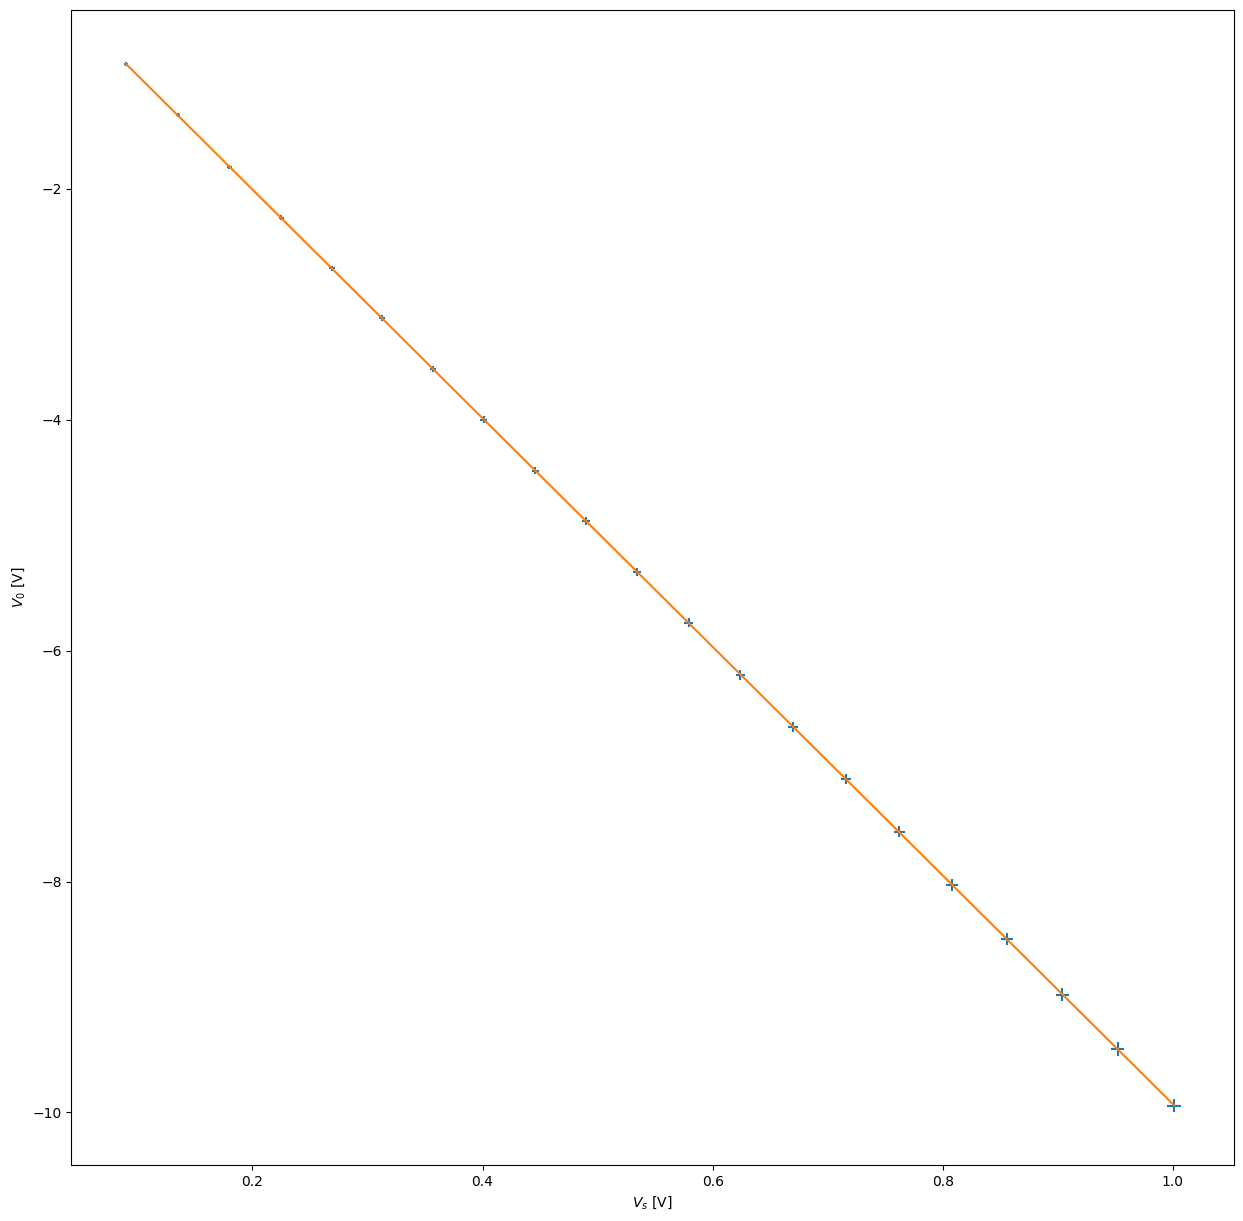
\includegraphics[width=1\textwidth]{fit-amplificatore.png}
    \caption{Fit lineare}
\end{figure} \noindent


\clearpage
\section{Parte 2}
\subsection{Determinazione della corrente di bias dell'amplificatore}
Il circuito è stato modificato rispetto alla fase precedente dell'esperienza: la resistenza di retroazione sul terminale invertente è stata sostituita da un condensatore di capacità 4.7 nF; in parallelo al condensatore abbiamo collegato una resistenza di retroazione sufficientemente grande (circa 100 KOhm); al terminale invertente è stata inoltre rimossa la resistenza $R_s$ con la relativa alimentazione fornita dal generatore a singolo canale e la conseguente regolazione tramite potenziometro multigiro. Il trimmer, precedentemente utilizzato, non è stato rimosso o modificato così da ottenere una misura di $V_o$ con un $V_{off}$ ridotto al minimo.
La configurazione del circuito è dunque la seguente
\begin{center}
    \begin{circuitikz}[scale=1.2, transform shape, thick]

    % Nodo di massa e linea verticale principale a sinistra
    \draw (-5, -1.5) node[ground]{} -- (-5, 0.5);

    % Box del circuito integrato (IC)
    \draw[rounded corners=3pt] (-1.5, -2.2) rectangle (1.5, 2.2);

    % Simbolo interno dell'Op-Amp
    \node[op amp] (oa) at (0, 0) {};
    \node[align=center, font=\scriptsize] at (-0.2, 0) {TL081};

    % Collegamenti dai pin interni dell'Op-Amp ai bordi dell'IC
    \draw (oa.-) -- (-1.5, 0.5);
    \draw (oa.+) -- (-1.5, -0.5);
    \draw (oa.out) |- (1.5, -0.5);

    % Etichette interne dei Pin dell'IC
    \node[right, font=\tiny] at (-1.5, 1.8) {1};
    \node[right, font=\scriptsize] at (-1.2, 1.8) {balance};
    \node[right=5pt, above = 2pt, font=\tiny] at (-1.5, 0.5) {2};
    \node[right=5pt, below = 2pt, font=\tiny] at (-1.5, -0.5) {3};
    \node[right, font=\tiny] at (-1.5, -1.8) {4};
    \node[right, font=\scriptsize] at (-1.2, -1.8) {$V^-$};

    \node[left, font=\tiny] at (1.5, 1.8) {8};
    \node[left, font=\scriptsize] at (1.2, 1.8) {N.C.};
    \node[left, font=\tiny] at (1.5, 0.5) {7};
    \node[left, font=\scriptsize] at (1.2, 0.5) {$V^+$};
    \node[left=5pt, below = 2pt, font=\tiny] at (1.5, -0.5) {6};
    \node[left, font=\tiny] at (1.5, -1.8) {5};
    \node[left, font=\scriptsize] at (1.2, -1.8) {balance};

    % Connessione Pin 3 a massa
    \draw (-1.5, -0.5) -- (-5, -0.5);
    \filldraw (-5, -0.5) circle (1.5pt);

    % Nodo e derivazione da Pin 2 ($R_s$ e Feedback)
    \draw (-1.5, 0.5) -- (-2.5, 0.5);
    \filldraw (-2.5, 0.5) circle (1.5pt);

    % $R_s$ verso la linea di massa
    \draw (-5, 0.5) to[R, l=$R_s$]  (-3.8, 0.5) -- (-2.5, 0.5);

    % Linea verticale sinistra del feedback
    \draw (-2.5, 0.5) -- (-2.5, 3.5);

    % Resistenza $R_f$ (Feedback)
    \draw (-2.5, 3.5) to[R, l=$R_f$] (3.5, 3.5);

    % Linea verticale destra del feedback e connessione a Pin 6
    \draw (3.5, 3.5) -- (3.5, -0.5);
    \draw (1.5, -0.5) -- (3.5, -0.5);
    \filldraw (3.5, -0.5) circle (1.5pt);

    % 7. Alimentazione Duale \pm 15V
    \draw (6.5, -0.5) to[battery] (6.5, -1.5) to[battery] (6.5, -2.5);
    \draw (6.5, -1.5) -- (7.5, -1.5) node[ground] (7.5, -2) {};
    \node[left] at (6.2, -1) {$+ 15V$};
    \node[left] at (6.2, -2) {$- 15V$};
    \filldraw (6.5, -1.5) circle (1.5pt);

    % Connessione V+ (Pin 7) con "salto" ad arco sopra il filo verticale del feedback
    \draw (1.5, 0.5) -- (3.3, 0.5) arc[radius=0.2, start angle=180, end angle=0] -- (6.5, 0.5) -- (6.5, -0.5);

    % Connessione V- (Pin 4) e diramazione (verso batteria a dx e trimmer in basso)
    \draw (-1.5, -1.8) -- (-1.5, -3.0);
    \filldraw (-1.5, -3.0) circle (1.5pt);
    \draw (-1.5, -3.0) -- (6.5, -3.0) -- (6.5, -2.5);

    % Trimmer a vite (rappresentato come resistore con cursore)
    \draw (-2.5, -4.5) to[R] (-0.5, -4.5) -- (2.5, -4.5);
    \node[align=center, below=0.2cm] at (-1.5, -4.6) {Trimmer\\a vite};
    
    % Cursore del trimmer dal nodo V-
    \draw[-latex] (-1.5, -3.0) -- (-1.5, -4.2);

    % Pin 1 (Balance sx): discesa con salti ad arco sopra il filo di $R_s$ e il filo di massa
    \draw (-1.5, 1.8) -- (-3.5, 1.8) -- (-3.5, 0.7)
          arc[radius=0.2, start angle=90, end angle=270] % Salto $R_s$
          -- (-3.5, -0.3)
          arc[radius=0.2, start angle=90, end angle=270] % Salto Massa
          -- (-3.5, -4.5) -- (-2.5, -4.5);

    % Pin 5 (Balance dx): discesa con salto ad arco sopra il filo di V-
    \draw (1.5, -1.8) -- (2.5, -1.8) -- (2.5, -2.8)
          arc[radius=0.2, start angle=90, end angle=-90] % Salto V-
          -- (2.5, -4.5);

\end{circuitikz}
\end{center}

\subsection{Misure effettuate}
Una volta realizzato il circuito, abbiamo scaricato il condensatore mediante
Una volta configurato il circuito, si è scaricato il condensatore mediante una resistenza posta in parallelo $R_f$ , scelta in modo tale che la costante di tempo associata alla scarica risultasse trascurabile e che il processo potesse essere considerato istantaneo. Successivamente, rimosso il collegamento di scarica, la corrente di bias dell'amplificatore operazionale (non più bilanciata dalla retroazione resistiva) ha iniziato a caricare lentamente il condensatore, determinando una variazione della tensione di uscita $V_0$ nel tempo. Per caratterizzare tale fenomeno, la tensione $V_0$ è stata misurata a intervalli regolari di 10 secondi per una durata complessiva di 2 minuti e 10 secondi, utilizzando un multimetro impostato su fondo scala di 20 V. Dall'analisi dell'andamento di $V_0$ in funzione del tempo, e noto il valore della capacità $\mathcal{C}$, è stato possibile determinare la corrente di bias dell'operazionale, tramite la seguente relazione
\begin{align}
     V_o= - \frac{I_b}{\mathcal{C}} t
\end{align}
L'incertezza sulla corrente di bias è stata stimata mediante la propagazione degli errori, tenendo conto della tolleranza del condensatore e dell'incertezza sulla pendenza del fit: 
\begin{align}
    \frac{\Delta I_b}{I_b} = \frac{\Delta \mathcal{C}}{\mathcal{C}} + \frac{\Delta m}{m}
\end{align}
\begin{table}[H]
    \centering
    \caption{Misure con condensatore}
    \vspace{0.1cm}
    \begin{tabular}{@{} >{\centering\arraybackslash}p{2.5cm} >{\centering\arraybackslash}p{2.5cm} >{\centering\arraybackslash}p{2.5cm} >{\centering\arraybackslash}p{2.5cm} @{}}
        \toprule
        \multicolumn{2}{c}{\textbf{Tempo misura ed errore [s]}} & \multicolumn{2}{c}{\textbf{Tensione misurata ed errore [V]}}  \\
        \cmidrule(lr){1-2} \cmidrule(lr){3-4}
        0	&1	&0.030	&0.010 \\
        10	&1	&0.060	&0.010 \\
        20	&1	&0.090	&0.010 \\
        30	&1	&0.120	&0.011 \\
        40	&1	&0.150	&0.011 \\
        50	&1	&0.180	&0.011 \\
        60	&1	&0.200	&0.011 \\
        70	&1	&0.230	&0.011 \\
        80	&1	&0.260	&0.011 \\
        90	&1	&0.290	&0.011 \\
        100	&1	&0.320	&0.012 \\
        110	&1	&0.350	&0.012 \\
        120	&1	&0.380	&0.012 \\
        \bottomrule
    \end{tabular}
\end{table}


\subsection{Analisi dati}
Nella configurazione integratrice, la corrente di bias dell’amplificatore
operazionale carica il condensatore di retroazione, producendo una
variazione lineare nel tempo della tensione di uscita. il modello teorico
è descritto dalla relazione: 
\begin{align}
    V_o=- \frac{I_b}{\mathcal{C}} t
\end{align}
In fase di analisi dati, i punti sperimentali sono stati interpolati
mediante una retta del tipo $V_o=mt+q$ al fine di tener conto di
eventuali condizioni iniziali non perfettamente nulle.
Il parametro fisicamente rilevante per la determinazione
della corrente di Bias è la pendenza m.
\begin{figure}[H]
    \centering
    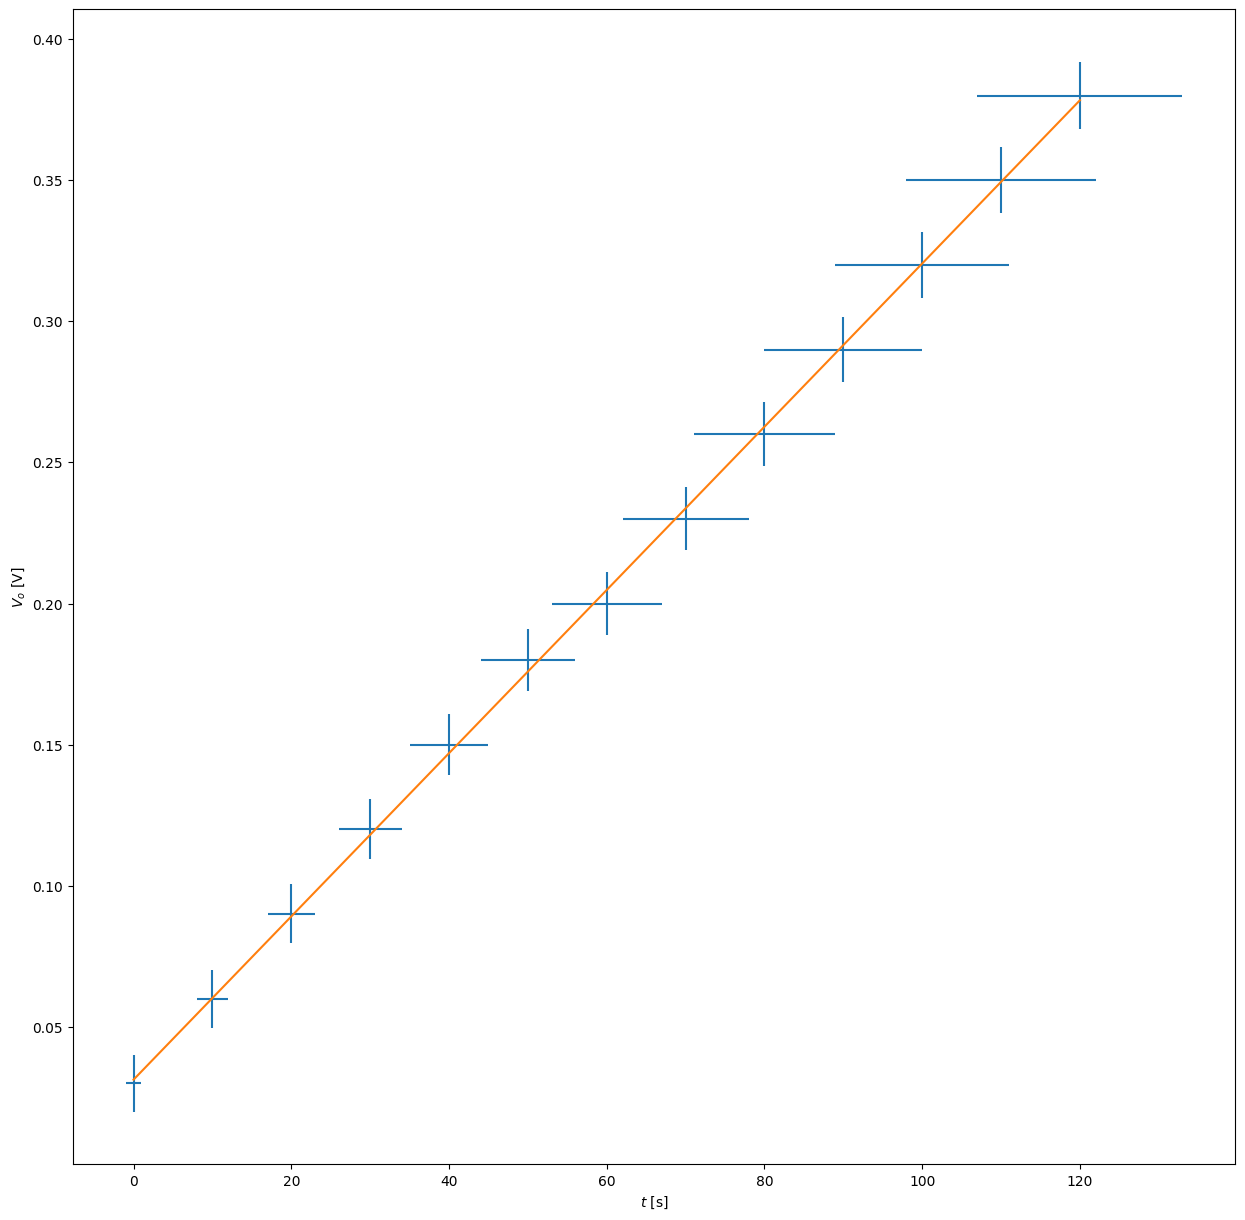
\includegraphics[width=0.75\textwidth]{fit-condensatore.png}
    \caption{Tensione in funzione del tempo}
\end{figure} \noindent
Dal fit lineare
si sono ottenuti:
\begin{itemize}
    \item $a \pm \Delta a = (0.00289 \pm 0.00002)$ A / F;
    \item $b \pm \Delta b = (0.0313 \pm 0.0009)$ V.
\end{itemize}
Utilizzando il valore della capacità del condensatore $\mathcal{C}$, si ricava la corrente di
Bias mediante
\begin{align}
    I_b = - m\mathcal{C}
\end{align}
da cui, in modulo,
\begin{align}
    I_b=(2.71\pm0.05)*10^{10} \qquad \qquad A=271\pm5\  \text{pA}.
\end{align} 
L’andamento lineare dei dati sperimentali conferma che,
nell’intervallo temporale considerato, il condensatore
viene caricato da una corrente approssimativamente
costante. Il valore ottenuto per la corrente di bias risulta
compatibile con l’ordine di grandezza atteso per un
operazionale a ingresso JFET, tenendo conto della
possibile presenza di contributi sistematici.


\section{Conclusioni}
L'esperienza ha consentito una caratterizzazione quantitativa del comportamento di un
amplificatore operazionale reale, mettendo in evidenza i limiti del modello ideale.
Nella configurazione invertente, il confronto tra guadagno teorico e sperimentale ha
mostrato una buona concordanza entro le incertezze sperimentali, confermando così la
validità del modello lineare $A_f$ in regime operativo. Tuttavia, la presenza
di un'intercetta non nulla ha evidenziato l'effetto (l'esistenza di una tensione di
offset, responsabile di uno scostamento sistematico della tensione di uscita.) sulla
tensione di offset $V_{off}$, che introduce un contributo sistematico sull'uscita.
La procedura di compensazione tramite trimmer ha permesso di ridurre
significativamente tale contributo, senza eliminarlo completamente
a causa di alcuni effetti residui. Questo aspetto sottolinea il
carattere intrinsecamente non ideale del dispositivo. 
Nella configurazione integratrice, l'evoluzione lineare della
tensione di uscita nel tempo ha fornito una misura indiretta
della corrente di bias $I_b$, confermando che anche correnti di
ordine estremamente ridotto possono produrre effetti macroscopicamente
osservabili in condizioni di elevata sensibilità circuitale, ulteriore
manifestazione della non idealità del circuito integrato. La coerenza
tra modello teorico e andamento sperimentale valida l'approccio utilizzato
per la stima di $I_b$.
Complessivamente, l'esperienza dimostra che le principali non idealità dell'amplificatore
operazionale non solo sono misurabili sperimentalmente ma influenzano in modo sistematico
il comportamento del circuito. La loro corretta identificazione e compensazione
rappresentano un aspetto fondamentale per un utilizzo consapevole e accurato
del dispositivo in applicazioni reali.

\end{document}